% \documentclass{book}

\documentclass[12pt]{article}
\usepackage[pdfborder={0 0 0.5 [3 2]}]{hyperref}%
\usepackage[left=1in,right=1in,top=1in,bottom=1in]{geometry}%
\usepackage[shortalphabetic]{amsrefs}%
\usepackage{amsmath}
\usepackage{enumerate}
\usepackage{enumitem}
\usepackage{amssymb}                
\usepackage{amsmath}                
\usepackage{amsfonts}
\usepackage{amsthm}
\usepackage{bbm}
\usepackage[table,xcdraw]{xcolor}
\usepackage{tikz}
\usepackage{float}
\usepackage{booktabs}
\usepackage{svg}
\usepackage{mathtools}
\usepackage{cool}
\usepackage{url}
\usepackage{graphicx,epsfig}
\usepackage{makecell}
\usepackage{array}

\graphicspath{ {images/} }

\def\noi{\noindent}
\def\T{{\mathbb T}}
\def\R{{\mathbb R}}
\def\N{{\mathbb N}}
\def\C{{\mathbb C}}
\def\Z{{\mathbb Z}}
\def\P{{\mathbb P}}
\def\E{{\mathbb E}}
\def\Q{\mathbb{Q}}
\def\ind{{\mathbb I}}

\begin{document}

\title{}
\author{\vspace{-10ex} }

\begin{center}
{\LARGE APMA 1650 -- Homework 6}\\
\vspace{5mm}
{\large Due Monday, July 25, 2016}\\
\vspace{5mm}
Homework is due during class or by 3:45 pm in the homework drop box in 182 George St.\\
Show all of your work used in deriving your solutions.
\end{center}

\begin{enumerate}

\item Suppose $X$ and $Y$ are discrete random variables with joint probability mass function given by:
\[
p(x, y) = \begin{cases}
\frac{1}{3} & (x, y) = (-1, 0), (0, 1), (1, 0) \\
\end{cases}
\]
(Recall that the discrete joint pmf specifies the probability for all pairs (x, y) which have positive probability. The three ordered pairs (x, y) above are the \emph{only} pairs (x,y) which have positive probability).
\begin{enumerate}
\item What is the covariance of $X$ and $Y$?\\

We will do this using the Magic Covariance Formula:
\[
Cov(X, Y) = \E(XY) - \E(X)\E(Y)
\]
First we find $\E(XY)$ using the pmf table above.
\begin{align*}
\E(XY) = (-1)(0)(1/3) + (0)(1)(1/3) + (1)(0)(1/3) = 0
\end{align*}
Using the pmf table above, we can also find the marginal distributions of $X$ and $Y$.
\begin{figure}[H]
\centering
\begin{tabular}{l@{\hskip 2cm}l}
\toprule
$x$ & $p_X(x)$\\
\midrule
-1 & 1/3\\
0 & 1/3\\
1 & 1/3\\
\bottomrule
\end{tabular}
\end{figure}

\begin{figure}[H]
\centering
\begin{tabular}{l@{\hskip 2cm}l}
\toprule
$y$ & $p_Y(y)$\\
\midrule
0 & 2/3\\
1 &1/3\\
\bottomrule
\end{tabular}
\end{figure}
We can use these to compute the expected values of $X$ and $Y$:
\begin{align*}
\E(X) &= -1 (1/3) + 0 (1/3) + 1 (1/3) = 0 \\
\E(Y) &=  0 (2/3) + 1 (1/3) = 1/3
\end{align*}
By the Magic Covariance Formula, $Cov(X, Y) = 0 - (0)(1/3) = 0$.

\item Are $X$ and $Y$ independent?

There are many ways to check that $X$ and $Y$ are not independent despite having a covariance of 0. One way is to note that $Y$ is a function of $X$, i.e. the value of $X$ completely determines $Y$. Alternatively, you can choose just about any $x$ and $y$ and show that $p(x,y)\neq p_X(x)p_Y(y)$.
\end{enumerate}

\item Let $X$ be a binomial random variable with parameters $n$ and $p$. Consider the following estimator for $p$:
\[
\hat{p}_1 = \frac{X+1}{n+2}
\]
\begin{enumerate}
\item Find the bias of $\hat{p}_1$.\\

By linearity of expectation,
\begin{align*}
\E(\hat{p}_1) &= \E\left( \frac{1}{n+2}X + \frac{1}{n+2} \right) \\
&= \frac{E(X)}{n+2} + \frac{1}{n+2}\\
&= \frac{np}{n+1} + \frac{1}{n+2}\\
&= \frac{np + 1}{n+2}
\end{align*}

Thus we have:
\begin{align*}
Bias(\hat{p}_1) &= \E(\hat{p}_1) - p \\
&= \frac{np + 1}{n+2} - p \\
&= \frac{np + 1 - p(n+2)}{n+2} \\
&= \frac{1 - 2p}{n+2}
\end{align*}

\item Find the mean square error (MSE) of $\hat{p}_1$.\\

Since the MSE is bias squared plus variance, it suffices to find the variance. Using the formula for the variance of $aX + b$,
\begin{align*}
Var(\hat{p}_1) &= Var\left( \frac{1}{n+2}X + \frac{1}{n+2} \right) \\
&= \frac{1}{(n+2)^2} Var(X) \\
&= \frac{np(1-p)}{(n+2)^2}
\end{align*}
Adding the bias squared and the variance, we get the MSE:
\begin{align*}
MSE(\hat{p}_1) &= \left( \frac{1 - 2p}{n+2} \right)^2 + \frac{np(1-p)}{(n+2)^2} \\
&= \frac{(1-2p)^2 + np(1-p)}{(n+2)^2}
\end{align*}

\item The standard, unbiased estimator for $p$ is 
\[
\hat{p} = \frac{X}{n}
\]
We computed the MSE of $\hat{p}$ in class. Does the standard, unbiased estimator $\hat{p}$ always have a lower MSE than the biased estimator $\hat{p}_1$. In other words, can you find a value of $p$ for which $MSE(\hat{p}_1) < MSE(\hat{p})$? (If you don't want to do this for generic $n$, feel free to choose whatever value of $n$ you want).\\

If the biased estimator ever has a lower MSE, it will likely be either on the extremes ($p = 0, p = 1$) or in the middle ($p$ = 1/2). The $p = 1/2$ case looks promising, since in that case the bias is actually 0. The standard estimator $\hat{p}$ is unbiased, so its MSE is equal to its variance. Taking $p = 1/2$, we have:
\[
MSE(\hat{p}) = Var\left(\frac{X}{n}\right) = \frac{np(1-p)}{n^2} = \frac{1}{4}\frac{n}{n^2}
\] 
For the biased estimator, taking $p = 1/2$, we have:
\begin{align*}
MSE(\hat{p}_1) = \frac{np(1-p)}{(n+2)^2} = \frac{1}{4}\frac{n}{(n+2)^2}
\end{align*}
This is smaller than the MSE of the standard estimator $\hat{p}$.
\end{enumerate}

\item The reading on a voltmeter is uniformly distributed over the interval $[\theta, \theta+1]$, where $\theta$ is the true voltage of the circuit. Using your voltmeter, you take $n$ consecutive voltage readings $Y_1, \dots, Y_n$ from a single circuit.
\begin{enumerate}
\item Show that the sample mean $\bar{Y}$ is a biased estimator for $\theta$, and compute the bias of $\bar{Y}$.\\

First we find the expected value of $\bar{Y}$. We know from class that $\E(\bar{Y} = \mu$, where $\mu$ is the population mean. Since the population has a uniform distribution, $\mu = (\theta + (\theta + 1)) / 2 = \theta + 1/2$. Since this is not $\theta$, our estimator is biased. The bias is $(\theta + 1/2) - \theta = 1/2$.

\item Find a function of $\bar{Y}$ which is an unbiased estimator of $\theta$.\\

To turn the expected value of $\bar{Y}$ into $\theta$, all we have to do is subtract 1/2. Thus $\bar{Y} - 1/2$ is an unbiased esimator for $\theta$.

\item Find the MSE of $\bar{Y}$ (the biased estimator) when $\bar{Y}$ is used as an estimator of $\theta$.\\

We have found the bias of $\bar{Y}$ so we only have to compute its variance. We know that $Var(\bar{Y}) = \sigma^2 / n$, where $\sigma^2$ is the population variance. Since this is a uniform distribution,
\[
\sigma^2 = \frac{((\theta + 1) - \theta)^2}{12} = \frac{1}{12}
\]
Thus the MSE is $(1/2)^2 + 1/12 = 1/3$.
\end{enumerate}

\item What do you know, another ACME widget factory question. In the last problem set, you had just launched a new line of MiniWidgets. In the intervening time, they have become so popular that your factory now has 10 machines devoted to producing MiniWidgets. The MiniWidgets produced by your machine have a mass which is normally distributed with a mean of 9 grams and a standard deviation of 0.2 grams.
\begin{enumerate}
\item On a routine inspection, you take a sample of 9 MiniWidgets produced by a single MiniWidget machine. You find that the average mass of the MiniWidgets in your sample is 8.85 grams. Do you think the MiniWidget machine is defective? (Hint: compute the probability that the sample mean is less than or equal to 8.85 grams).\\

Let $Y$ be the mass of one MiniWidget. Since the population has a normal distribution, the sample mean is normally distributed with mean 9 and standard deviation $0.2 / \sqrt{9} = 0.2 / 3  = 1/15$. Thus we have:
\begin{align*}
\P(Y \leq 8.85) &= \P \left( Z \leq \frac{8.85 - 9}{1/15} \right) \\
&= \P(Z \leq -2.25) \\
&= 0.0122
\end{align*}
Thus it is highly likely that something is wrong with the machine.

\item On another inspection, you find a machine which appears to be defective. You want to know the mean mass of widgets produced by that machine (population mean $\mu$). To determine this, you take a sample of widgets from the machine and compute the sample mean $\bar{Y}$. Assume this machine produces widgets that are normally distributed, and that the standard deviation is the same as the other machines. How many widgets do you need to sample to be 95\% confident that the sample mean is within 0.05 grams of the true population mean?\\

We can do this with the 68-95.99.7 rule. We want the true (population) mean to be within two (sample) standard deviations of the sample mean. Since we want two standard deviations of the sample mean to be 0.05, one standard deviation of the sample mean must be 0.025. Thus we solve:
\begin{align*}
\frac{\sigma}{\sqrt{n}} &= 0.025 \\
\sqrt{n} &= \frac{0.2}{0.025} = 8\\
n &= 64
\end{align*}
Thus we should sample 64 MiniWidgets.
\end{enumerate}

\item Take the unit circle (circle of radius 1) and inscribe it in a square. See the diagram below.

\begin{figure}[H]
\centering
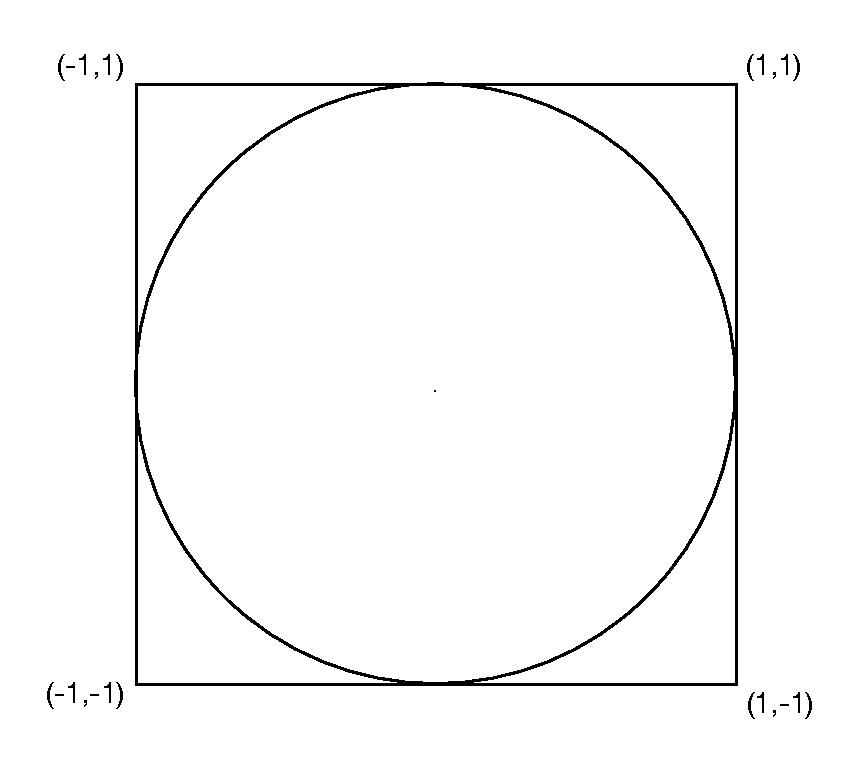
\includegraphics[width=6cm]{squarecircle.eps}
\end{figure}

You throw $n$ darts uniformly at random at the square. Let $Y$ be the number of darts which land in the circle. Form the estimator:
\[
\hat{\theta} = \frac{4Y}{n}
\]
What is the expected value of $\hat{\theta}$? What is $\hat{\theta}$ an estimator for?\\

$Y$ is the number of darts landing in the circle. The probability that a dart lands in the circle is the ratio of the circle area to the square area, which is $p = \pi / 4$. Thus $Y \sim $Binomial($n, \pi/4$). Thus we have
\[
\E(\hat{theta}) = \E\left( \frac{4Y}{n}\right) = \frac{4}{n} \E(Y) = \frac{4np}{n} = 4 \frac{\pi}{4} = \pi
\]
Thus this is an estimator for $\pi$. Alternatively, it is an estimator for the area of a circle.

\end{enumerate}

\end{document}

